\section{Processi organizzativi}
    \subsection{Gestione processi}
		\subsubsection{Scopo}
		Lo scopo della gestione dei processi è di migliorare l'organizzazione e la cooperazione tra i membri del \glo{Gruppo}{gruppo}. La corretta implementazione del processo deve:
		\begin{itemize}
			\item stabilire le modalità di comunicazione del \glo{Gruppo}{gruppo};
			\item definire i ruoli ed i compiti specifici;
			\item fornire la documentazione su strumenti di organizzazione e relative procedure.
		\end{itemize}
        \subsubsection{Comunicazioni}
            \paragraph{Interne}
                Per la comunicazione interna dei membri del \glo{Gruppo}{gruppo}, viene utilizzata l'applicazione \glo{Slack}{Slack} descritta in maniera piu dettagliata nella sezione \ref{sec:Slack}.
            \paragraph{Esterne}
				Per le comunicazioni esterne è stata creata la seguente mail:
				\begin{center}
					\mailzep
				\end{center}
				Il \responsabilediprogetto{} è la persona incaricata a inviare comunicazioni con questo indirizzo. Tutte le mail ricevute verranno inoltrate automaticamente ad ogni membro del \glo{Gruppo}{gruppo} a titolo informativo.
					% da valutare se inserire il canale \glo{Slack}{slack} + il reindirizzamento alla persona specifica di riskapp
        \subsubsection{Incontri}
            \paragraph{Interni}
            Il \responsabilediprogetto{} ha il compito di organizzare gli incontri interni rispettando la procedura descritta nella sezione \ref{sec:incontri_interni} .
	        Qualsiasi membro del \glo{Gruppo}{gruppo} può richiedere un incontro interno. Sarà compito del \responsabilediprogetto{} accettare o rifiutare la richiesta.
        	Al termine dell'incontro deve essere redatto un verbale, di cui si rimanda alla sezione \ref{sec:verbali} per la sua composizione in dettaglio.
            \paragraph{Esterni}
            Il \responsabilediprogetto{} ha il compito di organizzare gli incontri esterni con il proponente o committente seguendo la procedura descritta nella sezione \ref{sec:incontri_esterni}.
            Qualsiasi membro del \glo{Gruppo}{gruppo} può richiedere un incontro esterno. Sarà compito del \responsabilediprogetto{} accettare o rifiutare la richiesta.
            Al termine dell'incontro deve essere redatto un verbale, di cui si rimanda alla sezione \ref{sec:verbali} per la sua composizione in dettaglio.
        \subsubsection{Ruoli di progetto}
        	Ogni componente del \glo{Gruppo}{gruppo} deve ricoprire almeno una volta ciascuno dei ruoli previsti nello sviluppo del progetto. Nel \pdp{} vengono assegnati  compiti e ruoli che i membri del \glo{Gruppo}{gruppo} si impegnano a rispettare. Di seguito sono elencati i diversi incarichi, delineando per ciascuno mansioni e responsabilità.
			\paragraph{Responsabile di progetto}
			Il \responsabilediprogetto{} è la figura che rappresenta il \glo{Gruppo}{gruppo} e il progetto presso committente e proponente. Approva le scelte prese dal \glo{Gruppo}{gruppo} e se ne assume la responsabilità. La sua presenza segue tutta la durata del progetto.
			Le sue responsabilità sono:
			\begin{itemize}
				\item gestione delle risorse;
				\item approvazione della documentazione di progetto;
				\item analisi e mitigazione dei rischi;
				\item coordinamento e pianificazione delle attività di progetto seguendo il \pdp{}.
			\end{itemize}
			\paragraph{Amministratore di progetto}
			L'\amministratore{} è responsabile dell'ambiente di lavoro del \glo{Gruppo}{gruppo}, ne controlla l'efficienza e l'operatività.
			Le sue principali responsabilità sono:
			\begin{itemize}
				\item controllo delle versioni e configurazioni del prodotto;
				\item gestione del versionamento e dell'archiviazione della documentazione;
				\item risoluzione dei problemi inerenti la gestione di processi e risorse;
				\item controllo e miglioramento degli strumenti di lavoro e dell'infrastruttura;
				\item redazione e aggiornamento delle \ndp{}.
			\end{itemize}
			\paragraph{Analista}
			L'\analista{} ha il compito di esaminare e studiare attentamente il dominio del problema, la sua presenza non è necessaria per tutta la durata del progetto.
			Le sue responsabilità sono:
			\begin{itemize}
				\item capire il dominio di lavoro del cliente;
				\item analizzare e capire la natura del problema posto dal cliente;
				\item redigere lo studio di fattibilità e l'analisi dei requisiti.
			\end{itemize}
			\paragraph{Progettista}
			Il \progettista{} è responsabile di tutto ciò che riguarda la progettazione software. Deve avere conoscenze tecniche e tecnologiche aggiornate per la gestione del progetto.
			Le sue responsabilità sono:
			\begin{itemize}
				\item fornire una soluzione attuabile entro i limiti di tempo;
				\item descrivere il funzionamento del sistema a diversi livelli di dettaglio;
				\item effettuare scelte su aspetti tecnici del progetto, rendendolo efficiente, robusto e manutenibile.
			\end{itemize}
			\paragraph{Programmatore}
			Il \programmatore{} si occupa dell'attività di codifica. Le sue responsabilità sono:
			\begin{itemize}
				\item implementare le scelte dettate dal \progettista{}, senza apportare modifiche personali;
				\item documentare il codice prodotto;
				\item rispettare le convenzioni riportate nel presente documento;
				\item realizzare strumenti per verifica e validazione.
			\end{itemize}
			\paragraph{Verificatore}
			Il \verificatore{} è responsabile dell'attività di verifica. Deve avere una profonda conoscenza delle \ndp{} ed è presente per tutta la durata del progetto. Le sue responsabilità sono:
			\begin{itemize}
				\item controllare l'osservazione delle \ndp{} lungo tutte le attività del progetto stesso.
			\end{itemize}
        \subsubsection{Procedure}
	        \paragraph{Organizzazione incontri interni}
	        \label{sec:incontri_interni}
	        L'organizzazione degli incontri interni deve essere svolta rispettando il seguente ordine:
	        \begin{enumerate}
	        	\item controllare il foglio condiviso su \glo{Google Drive}{Google Drive} \textit{Orari impegni ricorrenti};
	        	\item postare sul canale \glo{Slack}{Slack} \textit{\#incontri-interni} alcune proposte di incontro, indicando: luogo, data e orario;
	        	\item assicurarsi che tutti i membri del \glo{Gruppo}{gruppo} abbiano espresso la preferenza, in caso contrario entro 24 ore, contattarli telefonicamente;
	        	\item aggiungere l'evento nel calendario di \glo{Teamwork}{Teamwork} con le seguenti caratteristiche:
	        	\begin{itemize}
	        		\item \textbf{titolo evento:} Riunione interna;
	        		\item \textbf{dove:} data, ora inizio, ora fine;
	        		\item \textbf{dettagli:} luogo concordato, breve descrizione degli argomenti da trattare;
	        		\item \textbf{persone:} assegnare i partecipanti;
	        		\item \textbf{reminders:} assegnare dei promemoria se lo si ritiene necessario.
	        	\end{itemize}
	        \end{enumerate}
	        \paragraph{Organizzazione incontri esterni}
	        \label{sec:incontri_esterni}
	        L'organizzazione degli incontri esterni deve essere svolta rispettando il seguente ordine:
	         \begin{enumerate}
		        \item contattare il proponente per avere informazioni sulla sua disponibilità;
		        \item postare sul canale \glo{Slack}{Slack} \textit{\#incontri-esterni}{} alcune proposte di incontro, indicando: luogo, data e orario;
		        \item assicurarsi che tutti i membri del \glo{Gruppo}{gruppo} abbiano espresso la preferenza, in caso contrario entro 24 ore, contattarli telefonicamente;
		        \item aggiungere l'evento nel calendario di \glo{Teamwork}{Teamwork} con le seguenti caratteristiche:
		        \begin{itemize}
		        	\item \textbf{Titolo evento:} Riunione esterna;
		        	\item \textbf{Dove:} data, ora inizio, ora fine;
		        	\item \textbf{Dettagli:} luogo concordato, breve descrizione degli argomenti da trattare;
		        	\item \textbf{Persone:} assegnare i partecipanti;
		        	\item \textbf{Reminders:} assegnare dei promemoria se lo si ritiene necessario.
		        \end{itemize}
	        \end{enumerate}
            \paragraph{Gestione dei ticket}
            Accedere allo spazio \glo{Teamwork}{Teamwork} del \glo{Gruppo}{gruppo}, posizionandosi nella sezione \textit{"All Task"} oppure tramite il seguente link: \url{https://swe2016.teamwork.com/#projects/140646/tasks}. Premere su \textit{"Add Task"} per la creazione o sul nome di un task già esistente per la modifica.
            \subparagraph{Creazione di un ticket}\label{sec:creazioneticket}
                La creazione di un ticket deve essere svolta rispettando il seguente ordine:
                \begin{enumerate}
                	\item inserimento titolo task;
                	\item assegnazione delle persone incaricate al suo svolgimento;
                	\item inserimento data prevista di completamento;
                	\item inserimento descrizione;
                	\item inserimento priorità;
                	\item selezionare eventuali dipendenze da altri task;
                	\item inserimento di un \glo{Tag}{tag} che identifichi il ruolo delle persone incaricate;
                	\item salvataggio task.
                \end{enumerate}
                Vedi figura \ref{fig:procassticket}.
    	        \begin{figure}[h!]
    		        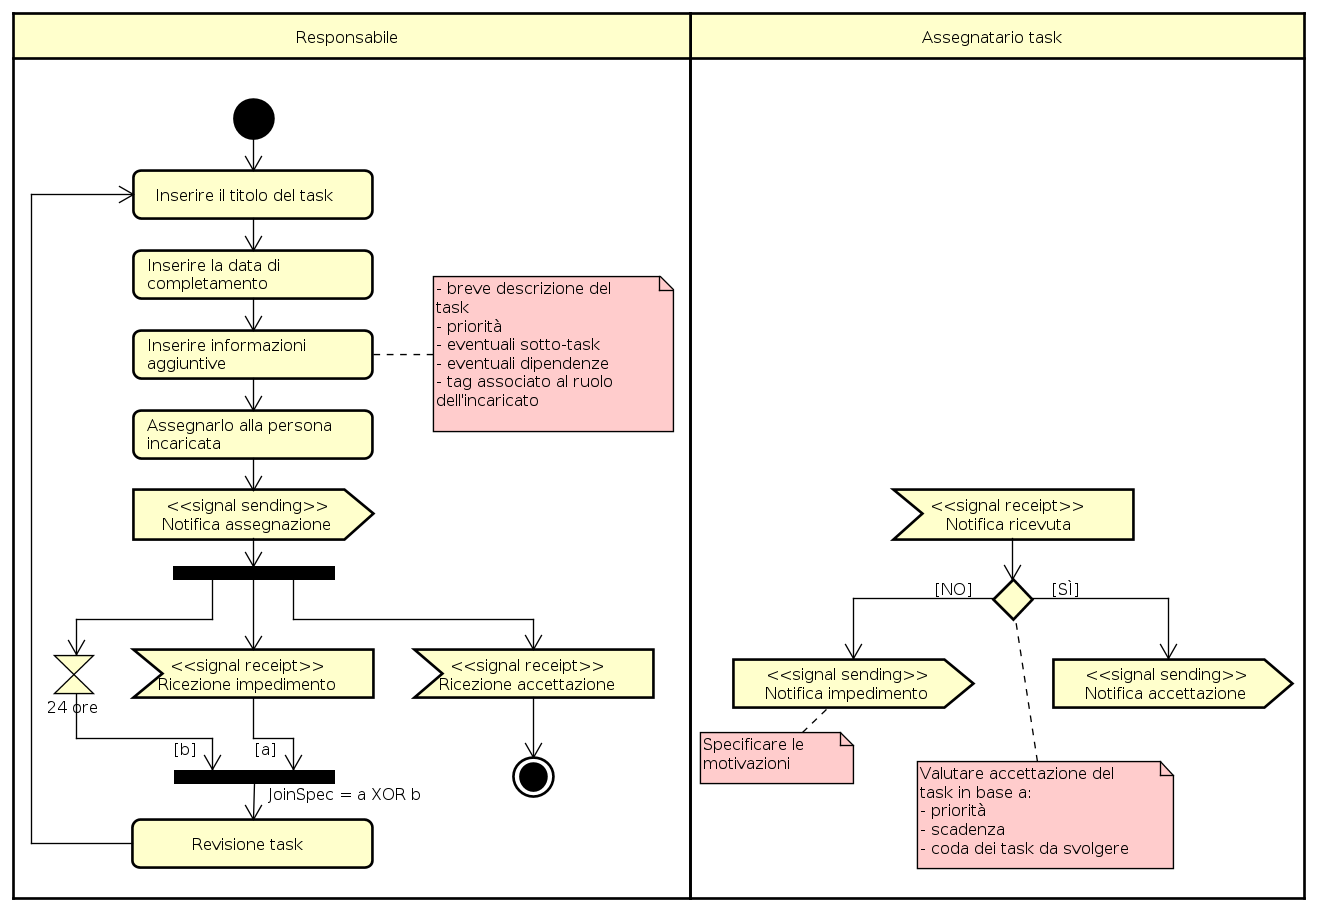
\includegraphics[width=\textwidth]{img/proc_ass_ticket.png}
    		        \captionof{figure}{Procedura assegnazione ticket. Riferita nella sezione \ref{sec:creazioneticket}}
                    \label{fig:procassticket}
    	        \end{figure}\mbox{}\\
            \subparagraph{Modifica di un ticket}\label{sec:modificaticket}
                La modifica di un ticket deve essere svolta rispettando il seguente ordine:
                \begin{enumerate}
                	\item ricerca del ticket da modificare;
                	\item modifica di uno o più campi;
                	\item verifica inserimento dei campi dati: titolo, assegnatario, descrizione e data di completamento;
                	\item salvare le modifiche apportate.
                \end{enumerate}
                Vedi figura \ref{fig:procmodticket}.
                    \begin{figure}[h!]
                        \centering
        	        	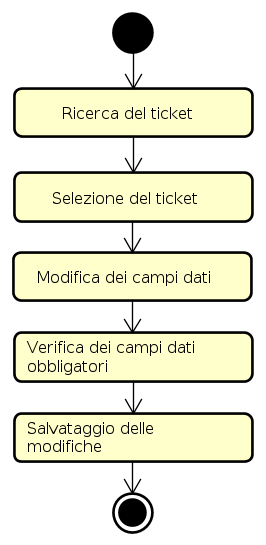
\includegraphics[width=0.3\textwidth]{img/proc_mod_ticket}
                        \captionof{figure}{Procedura modifica ticket. Riferita nella sezione \ref{sec:modificaticket}}
                        \label{fig:procmodticket}
        	        \end{figure}\mbox{}\\
            \paragraph{Gestione delle milestone}
            Accedere allo spazio \glo{Teamwork}{Teamwork} del \glo{Gruppo}{gruppo}, posizionandosi nella sezione \textit{"Milestones"} oppure tramite il seguente link: \url{https://swe2016.teamwork.com/#/projects/140646/milestones/upcoming}. Premere su \textit{"Add \glo{Milestone}{Milestone}"} per la creazione o sul nome di una \glo{Milestone}{milestone} esistente per la modifica.
            \subparagraph{Creazione milestone}\label{sec:creazionemilestone}
                La creazione di una \glo{Milestone}{milestone} deve essere svolta rispettando il seguente ordine:
    			\begin{enumerate}
    				\item inserimento titolo \glo{Milestone}{milestone};
    				\item inserimento data;
    				\item assegnazione persone coinvolte;
    				\item assegnazione reminders;
    				\item inserimento descrizione;
    				\item salvataggio \glo{Milestone}{milestone}.
    			\end{enumerate}
                Vedi figura \ref{fig:procinsmilestone}.
    			\begin{figure}[h!]
                    \centering
    				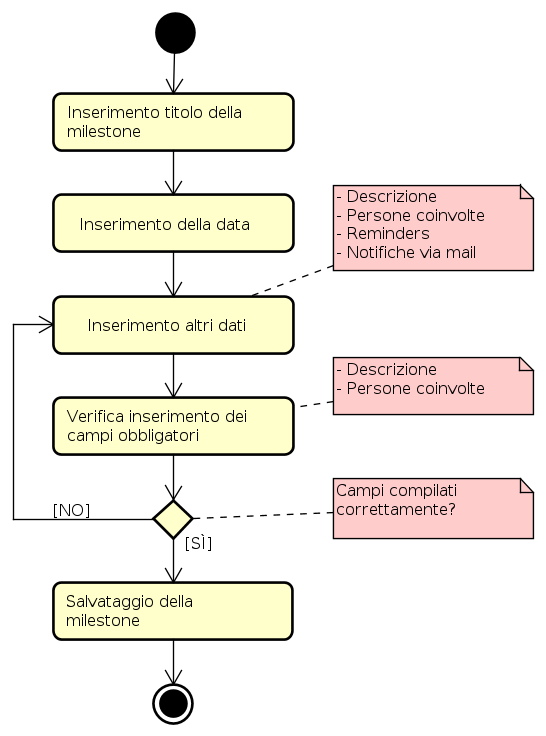
\includegraphics[width=0.5\textwidth]{img/proc_ins_milestone}
    				\captionof{figure}{Procedura inserimento \glo{Milestone}{milestone}. Riferita nella sezione \ref{sec:creazionemilestone}}
                    \label{fig:procinsmilestone}
    			\end{figure}\mbox{}\\
            \subparagraph{Modifica milestone}\label{sec:modificamilestone}
			La modifica di una \glo{Milestone}{milestone} deve essere svolta rispettando il seguente ordine:
    			\begin{itemize}
    				\item selezione \glo{Milestone}{milestone};
    				\item modifica di uno o più campi dati;
    				\item verifica inserimento dei campi dati: titolo, data, descrizione e assegnatari;
    				\item salvataggio \glo{Milestone}{milestone}.
    			\end{itemize}
                Vedi figura \ref{fig:procmodmilestone}.
        		\begin{figure}[h!]
                    \centering
        			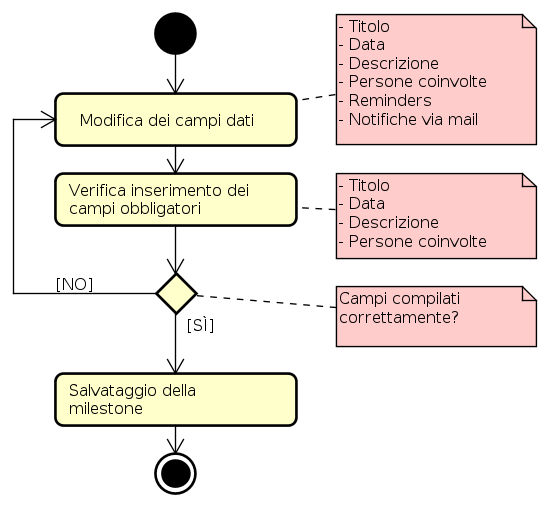
\includegraphics[width=0.5\textwidth]{img/proc_mod_milestone}
        			\captionof{figure}{Procedura modifica \glo{Milestone}{milestone}. Riferita nella sezione \ref{sec:modificamilestone}}
                    \label{fig:procmodmilestone}
        		\end{figure}\mbox{}\\
        \subsubsection{Strumenti}
            \paragraph{Slack}
	        \label{sec:Slack}
            \glo{Slack}{Slack} è un servizio gratuito  di messaggistica professionale disponibile su piattaforme mobile, desktop e web. Le principali motivazioni che hanno portato il \glo{Gruppo}{gruppo} alla scelta di questo strumento sono:
            \begin{itemize}
            	\item possibilità di integrazione con molti servizi (tra i principali: \glo{Dropbox}{Dropbox}, \glo{GitHub}{GitHub}, GoogleDrive, bot etc.);
            	\item possibilita di creazione di canali tematici personalizzati con la profilazione delle utenze e delle notifiche;
            	\item utilizzato come ulteriore canale per comunicare con \riskapp{} in quanto anche loro lo utilizzano;
            	\item possibilita di richiamare all'attenzione un membro del \glo{Gruppo}{gruppo} con il comando "@";
            	\item possiblità di classificare  un commento  come "rilevante" tramite il comando "pin to";
            	\item possibilità di inserire dei reminder sui messaggi;
            	\item \glo{Cross-platform}{cross-platform} e \glo{Cross-device}{cross-device};
            	\item interfaccia piu ricca e organizzata rispetto alle usuali applicazioni di messaggistica.
            \end{itemize}
            Lo spazio dedicato al \glo{Gruppo}{gruppo} si trova al seguente indirizzo:
            \begin{center}
            	\url{https://zephyrus-swe.slack.com/home}
            \end{center}
            \paragraph{Teamwork}\label{sec:teamwork}
            \glo{Teamwork}{Teamwork} è un'applicazione web di project management che permette di sfruttare le seguenti funzionalità principali:
            \begin{itemize}
            	\item gestione dei task;
            	\item gestione degli appuntamenti con scadenze a calendario;
            	\item pianificazione del lavoro;
            	\item rendiconto ore lavoro su intero progetto e/o su specifici task.
            \end{itemize}
            Le principali motivazioni che hanno portato il \glo{Gruppo}{gruppo} alla scelta di questo strumento sono:
            \begin{itemize}
            	\item le funzionalità essenziali sono gratuite;
            	\item alta portabilità ed accessibilità essendo fruibile via web;
            	\item interfaccia semplice e funzionale.
            \end{itemize}
            Lo spazio di lavoro dedicato al \glo{Gruppo}{gruppo} di trova al seguente indirizzo:
            \begin{center}
            	\url{https://swe2016.teamwork.com/}
            \end{center}
            \paragraph{Condivisione file}
            % 1)descrizione veloce dell'app
            \textit{\glo{Dropbox}{Dropbox}} è un servizio che offre la possibilità di salvare file su una piattaforma \glo{Cloud}{cloud} personale e mantenerli sincronizzati tra diversi dispositivi tramite un client.
            % 2)cosa ci permette di fare
            Il \glo{Gruppo}{gruppo} ha scelto \glo{Dropbox}{Dropbox} per gestire file che non necessitano versionamento,
            % 3) perche l'abbiamo scelta
            inoltre le principali motivazioni che ne hanno portato alla scelta sono:
            \begin{itemize}
            	\item alta velocità nella sincronizzazione dei file;
            	\item servizio già conosciuto e largamente utilizzato da tutti i membri del \glo{Gruppo}{gruppo};
            	\item lo spazio disponibile nella versione gratuita è sufficente per consentire una discreta quantità di file associati a questo progetto;
            	\item alta portabilità e usabilità essendo \glo{Cross-platform}{cross-platform} e \glo{Cross-device}{cross-device}.
            \end{itemize}
            % 4) indirizzo dove collegarsi
            Indirizzo per il download:
            \begin{center}
            	\url{https://www.dropbox.com}
            \end{center}
            % 1)descrizione veloce dell'app
            \textit{\glo{Google Drive}{Google Drive}} è un servizio \glo{Cloud}{cloud}, di memorizzazione e sincronizzazione online offerto da \textit{Google}. Il servizio comprende il \glo{File hosting}{file hosting}, il file sharing e la modifica collaborativa di documenti. Per accedere allo spazio condiviso è necessario che ogni membro sia prima aggiunto dal \responsabilediprogetto.
            % 2)cosa ci permette di fare
            Il \glo{Gruppo}{gruppo} ha scelto questo strumento per la possibilità di redigere documenti in maniera collaborativa come attività preliminare a fine organizzativo.
            % 3) perche l'abbiamo scelta
            Le principali motivazioni che hanno portato il \glo{Gruppo}{gruppo} alla scelta di questo strumento sono:
            \begin{itemize}
            	\item servizio già conosciuto e utilizzato da tutti i membri del \glo{Gruppo}{gruppo};
            	\item gratuito;
            	\item alta portabilità e usabilità essendo \glo{Cross-platform}{cross-platform} e \glo{Cross-device}{cross-device}.
            \end{itemize}
            % 4) indirizzo dove collegarsi
            Lo spazio di lavoro dedicato al \glo{Gruppo}{gruppo} di trova al seguente link:
            \begin{center}
            	\href{https://drive.google.com/drive/folders/0Bzwj6VVb_wEeYkhoYkdzVW5qQnM?usp=sharing}{Google Drive Zephyrus}
            	% da valutare se inserire, xk si vede tutto, xò se un membro del \glo{Gruppo}{gruppo} deve accedere al \glo{Gruppo}{gruppo} su drive come farebbe? al limite mettere il link alla pagina drive "generica"
            \end{center}

    \subsection{Gestione delle infrastrutture}
        \subsubsection{Scopo}
        Lo scopo del processo di gestione delle infrastrutture è di stabilire e mantenere le infrastrutture e gli strumenti necessari allo svolgimento dei processi durante lo svolgimento del progetto. La corretta implementazione del processo deve:
        \begin{itemize}
            \item fornire un ambiente di lavoro idoneo;
            \item garantire il funzionamento di tutte le infrastrutture necessarie;
            \item indicare il corretto utilizzo delle infrastrutture.
        \end{itemize}
        \subsubsection{Struttura dei repository}
        Il \glo{Gruppo}{gruppo} ha scelto di utilizzare \glo{GitHub}{GitHub} per il versionamento e il salvataggio dei file inerenti le attività di progetto. L'\amministratore{} di progetto deve creare e organizzare i \glo{Repository}{repository} necessari e assicurarsi che tutti i membri del \glo{Gruppo}{gruppo} vi possano accedere. Ogni membro deve essere registrato su \glo{GitHub}{GitHub} e aver attivato l'account studente.
        \newline \newline
        Il \glo{Repository}{repository} dedicato ai documenti si trova al seguente indirizzo:
        \begin{center}
        	\url{https://github.com/JordanGottardo/Documenti}
        \end{center}
        Il \glo{Repository}{repository} dedicato al codice si trova al seguente indirizzo:
        \begin{center}
        	\url{https://github.com/JordanGottardo/DeGeOp}
        \end{center}
        Le cartelle nel \glo{Repository}{repository} vengono organizzate nel seguente modo a partire dalla root:
        \begin{itemize}
        	\item \textbf{documenti:} sono presenti le cartelle per ogni \glo{Fase}{fase} del progetto:
	        \begin{itemize}
	        	\item \textbf{01-RR}: contenente i documenti e i file le necessari alla \revereq;
	        	\item \textbf{02-RP}: contenente i documenti e i file le necessari alla \revprog;
	        	\item \textbf{03-RQ}: contenente i documenti e i file le necessari alla \revaqual;
		        \item \textbf{04-RA}: contenente i documenti e i file le necessari alla \revacc;
                \item \textbf{Script}: contenente script e altri strumenti utili per la stesura e la verifica dei documenti;
		        \item \textbf{Template}: contenente i file del template da usare per la creazione dei documenti \LaTeX.
	        \end{itemize}
	        \item \textbf{codice}: la descrizione di questa cartella verrà fornita in una \glo{Fase}{fase} successiva di lavoro.
        \end{itemize}
        \subsubsection{Nomi dei file}
        I nomi dei documenti presenti nel \glo{Repository}{repository} devono rispettare la notazione \glo{Camel case}{camel case} con le seguenti caratteristiche:
        \begin{itemize}
        	\item la prima lettera di ogni file è maiuscola, le successive minuscole fino al presentarsi della parola successiva che inizia con la lettera maiuscola e cosi via;
        	\item è possibile utilizzare unicamente caratteri alfanumerici e il trattino basso;
        	\item i nomi non possono contenere spazi o elementi di punteggiatura.
        \end{itemize}
        \subsubsection{Messaggi di commit}
		Ogni volta che si effettuano modifiche sui file del \glo{Repository}{repository} locale per poi esser caricate in quello remoto, bisogna specificarne le motivazioni. Per uniformare l'ambiente di lavoro è stato scelto un formato standard per la scrittura di una \glo{Commit}{commit}. Si veda la sezione \ref{commit} per il dettaglio sulla procedura da seguire.
        \subsubsection{Procedure}
            \paragraph{Installazione e configurazione di Git}
            L'installazione di \glo{Git}{Git} varia a seconda del sistema operativo utilizzato. Di seguito verranno elencate le principali procedure d'installazione.
            \newline \newline
            Per i sistemi \glo{Linux}{Linux}:
            \begin{itemize}
            	\item aprire il terminale;
            	\item eseguire il comando sudo \texttt{apt-get update};
            	\item eseguire il comando \texttt{apt-get install \glo{Git}{git}}.
            \end{itemize}
            Per i sistemi \glo{Windows}{Windows}:
            \begin{itemize}
            	\item accedere al sito ufficiale \url{https://git-scm.com/download/win};
            	\item scaricare l'eseguibile;
            	\item installare l'eseguibile seguendo la procedura guidata.
            \end{itemize}
    	    Per i sistemi \glo{MacOS}{MacOS}:
    	    \begin{itemize}
    	    	\item accedere al sito ufficiale \url{https://git-scm.com/download/mac};
    	    	\item scaricare l'eseguibile;
    	    	\item aprire il file appena scaricato e avviare l'installazione cliccando sul file \texttt{.pkg}.
    	    \end{itemize}
    	    La configurazione iniziale prevede l'inserimento del nome dell'utente e la connessione con l'account \glo{GitHub}{GitHub} tramite la seguente procedura:
    	    \begin{itemize}
    			\item \texttt{{git} config --global user.name <Nome Cognome>}: imposta il nome dell'utente, che comparirà come autore delle \glo{Commit}{commit} effettuate;
    			\item \texttt{{git} config --global user.email <email>}: imposta l'email dell'utente; deve essere impostata la stessa email utilizzata per la registrazione su \glo{GitHub}{GitHub}.
    		\end{itemize}
    		Per la creazione di una cartella locale del \glo{Repository}{repository} si deve seguire la seguente procedura:
    		\begin{itemize}
    			\item creare una nuova cartella;
    			\item aprire il terminale;
    			\item posizionarsi all'interno della cartella precedentemente creata;
    			\item eseguire il comando: \texttt{git init};
    			\item recuperare l'indirizzo URL del progetto su \glo{GitHub}{GitHub};
    			\item eseguire il comando: \texttt{git clone <indirizzo appena recuperato>}.
    		\end{itemize}

            \paragraph{Invio di commit}
            \label{commit}
    		Il comando \texttt{\glo{Commit}{commit}} adibito all'esecuzione dell'omonima operazione, deve essere composto da un messaggio riassuntivo delle operazioni svolte e una breve descrizione contenente:
    		\begin{itemize}
    			\item lista dei file coinvolti;
    			\item lista delle modifiche effettuate per ogni file.
    		\end{itemize}
    		\paragraph{Comandi utili Git}
    		Per l'approfondimento dei principali comandi riguardanti l'utilizzo di \glo{Git}{Git} è stata redatta una guida, consultabile al seguente indirizzo: \href{https://github.com/JordanGottardo/Documenti/blob/master/README.md}{Guida Git}.

    \subsubsection{Strumenti}
        \paragraph{Git}
        \glo{Git}{Git} è un \glo{Sistema di controllo di versione}{sistema software di controllo di versione} distribuito e \glo{Open source}{open source}. La versione utilizzata al momento della stesura di questo documento è la 2.11.0 o superiore.
        Le principali motivazioni che hanno portato il \glo{Gruppo}{gruppo} alla scelta di questo strumento sono:
        \begin{itemize}
        	\item largamente usato in ambito lavorativo;
        	\item performance superiori rispetto ad altri sistemi di versionamento;
        	\item sistema distribuito anziché centralizzato.
        \end{itemize}
        Indirizzo per il download e documentazione:
        \begin{center}
        	\url{https://git-scm.com}
        \end{center}
        L'utilizzo di \glo{Git}{Git} verrà effettuato tramite riga di comando. Si lascia libertà ai membri del \glo{Gruppo}{gruppo} per l'installazione di eventuali interfacce grafiche personalizzate.
        \paragraph{GitHub}
        \glo{GitHub}{GitHub} è un servizio di web di hosting per lo sviluppo di progetti software. Tra le caratteristiche principali:
        \begin{itemize}
        	\item utilizzo del \glo{Sistema di controllo di versione}{sistema di controllo di versione} \glo{Git}{Git};
        	\item oltre al codice sorgente è possibile inserire documentazione e immagini;
        	\item \glo{Issue}{issue} tracking;
        	\item funzionalità simili ai social network come follower, commenti e notifiche;
        	\item visione di grafici e statistiche su sviluppatori e \glo{Repository}{repository}.
        \end{itemize}
        Le principali motivazioni che hanno portato il \glo{Gruppo}{gruppo} alla scelta di questo strumento sono:
        \begin{itemize}
        	\item possibilità di creare \glo{Repository}{repository} private attivando il piano studente con l'email universitaria;
        	\item sistema largamente diffuso e conosciuto da alcuni membri del \glo{Gruppo}{gruppo};
        	\item integrabile con altre applicazioni (es: \glo{Slack}{Slack}, \glo{IDE}{IDE}).
        \end{itemize}
        \paragraph{Sistemi operativi}
        I membri del \glo{Gruppo}{gruppo} operano sui seguenti sistemi operativi:
        \begin{itemize}
            \item \glo{Linux}{Linux} distribuzioni: Debian v8.0, Ubuntu v16.04 e superiori, Mint v17.1;
            \item \glo{Windows}{Windows} versione: 10;
            \item \glo{MacOS}{MacOS} versione: 10.12.
        \end{itemize}

    \subsection{Apprendimento}
        \subsubsection{Scopo}
        Lo scopo del processo di apprendimento è di garantire che tutti i membri del \glo{Gruppo}{gruppo} abbiano conoscenze e capacità sufficienti per svolgere le attività assegnatagli. Nel caso in cui un componente del \glo{Gruppo}{gruppo} ritenga di non essere in grado di svolgere un task dovrà segnalarlo immediatamente al \responsabilediprogetto{} che dovrà organizzare le attività necessarie all'apprendimento.
